
\begin{block}{Named Entity Recognition}
\begin{table}[t]
  {\small
%% NER 
\begin{tabular}{l r r r r r r | r r r r r}
  \multicolumn{7}{c|}{Named Entity Recognition} & 
      \multicolumn{3}{c}{Face Identification} \\
      \textbf{System} & \textbf{Delay/tok} & \textbf{Qs/tok} & \textbf{PER F$_1$} & \textbf{LOC F$_1$} & \textbf{ORG F$_1$} & \textbf{F$_1$}
          & \textbf{Latency} & \textbf{Qs/ex} & \textbf{Acc.} 
    \\ \hline
    1-vote & 467 ms & 1.0 & 90.2 & 78.8 & 71.5 & 80.2
      & %1-vote & 
      1216 ms & 1.0 & 93.6 \\ %\hline
    3-vote & 750 ms & 3.0 & 93.6 & 85.1 & 74.5 & 85.4
        & %3-vote &
        1782 ms & 3.0 & 99.1 \\ %\hline
    5-vote & 1350 ms & 5.0 & \textbf{95.5} & 87.7 & 78.7 & 87.3 
        & 
        2103 ms & 5.0 & 99.8 \\ \hline
    Online & n/a & n/a & 56.9 & 74.6 & 51.4 & 60.9
        % Online 
        & n/a & n/a & 79.9 \\    %\hline
    Threshold & 414 ms & 0.61 & 95.2 & \textbf{89.8} & 79.8 & 88.3
        % threshold 
        & 1680 ms & 2.66 & 93.5 \\ %\hline
    \textbf{LENSE} & \textbf{267 ms} & \textbf{0.45} & 95.2 & 89.7 & \textbf{81.7} & \textbf{88.8} 
    %\textbf{LENSE} 
    & 1590 ms & 2.37 & 99.2 \\   %\hline
\end{tabular}
}
\caption{Results on NER and Face tasks comparing latencies, queries per token (Qs/tok)
and performance metrics (\fone{} for NER and accuracy for Face).}
\label{tbl:results}
\end{table}

  \begin{center}
    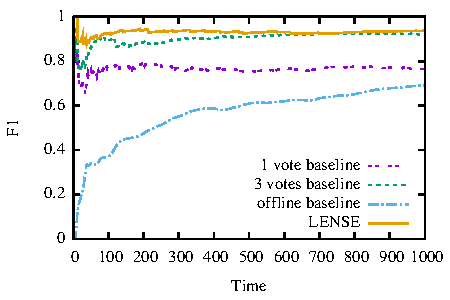
\includegraphics[width=0.45\columnwidth]{ner_2_class/f1_plot/f1_vs_time.pdf}
    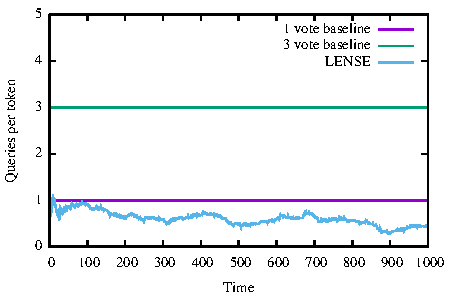
\includegraphics[width=0.45\columnwidth]{ner_2_class/cost_plot/cost_vs_time.pdf}
  \end{center}
\end{block}

\begin{block}{Sentiment}
\begin{table}[t]
    \begin{minipage}[t]{.45\textwidth}
  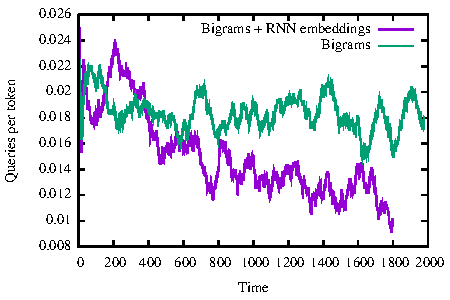
\includegraphics[width=\textwidth]{sentiment_cost_per_token_vs_time/cost_per_token_vs_time.pdf}
  \caption{Queries per example for LENSE on Sentiment. With simple \textsc{unigram} features, the model quickly learns it does not have the capacity to answer confidently and must query the crowd. With more complex \textsc{rnn} features, the model learns to be more confident and queries the crowd less over time.}
        \label{fig:sentiment-tradeoff}
    \end{minipage}
    \qquad
    \begin{minipage}[t]{.45\textwidth }
        \begin{tabular}[b]{l  r  r  r  r}
    %\hline
    \textbf{System} & \textbf{Latency} & \textbf{Qu./ex} & \textbf{Acc.} \\ \hline
    1-vote & 6.6 s & 1.00 & 89.2 \\ %\hline
    3-vote & 10.9 s & 3.00 & 95.8 \\ %\hline
    5-vote & 13.5 s & 5.00 & 98.7 \\ %\hline
    \multicolumn{5}{c}{\textsc{bigrams}} \\ \hline
%Bigrams: \\
    Offline & n/a & n/a & TODO \\ %\hline
    \textbf{Threshold} & TODO s & TODO & TODO \\ %\hline
    LENSE & 18.1 s & 3.48 & 98.6 \\ %\hline
    \multicolumn{5}{c}{\textsc{rnn}} \\ \hline
    Offline & n/a & n/a & TODO \\ %\hline
    \textbf{Threshold} & 11.0 s & 2.85 & 96.0 \\ %\hline
    \textbf{LENSE} & 16.1 s & 3.19 & 98.6 \\% \hline
\end{tabular}

        \caption{Results on the Sentiment task comparing latency, queries per example and accuracy.}
        \label{tbl:sentiment-results}
        \vfill
    \end{minipage}%
\end{table}

\end{block}


